\section{Architecture}
% Exemples de bon fonctionnement, schémas, justifications, explication de la décomposition modulaire (modules, classes, paquetages, namespaces), points techniques d'implémentation, utilisation de bibliothèques externes, extensions, application de principes logiciels.

Notre architecture est composée de cinq packages qui permettent à deux logiques distinctes de se compléter : Le moteur de jeu et l'IA.\\

Le moteur repose en grande partie sur le pattern Model/View/Controller.\\

% Mettre une vue d'ensemble de l'architecture avant de rentrer dans les sous-parties ?

\begin{figure}[H]
    \centering
    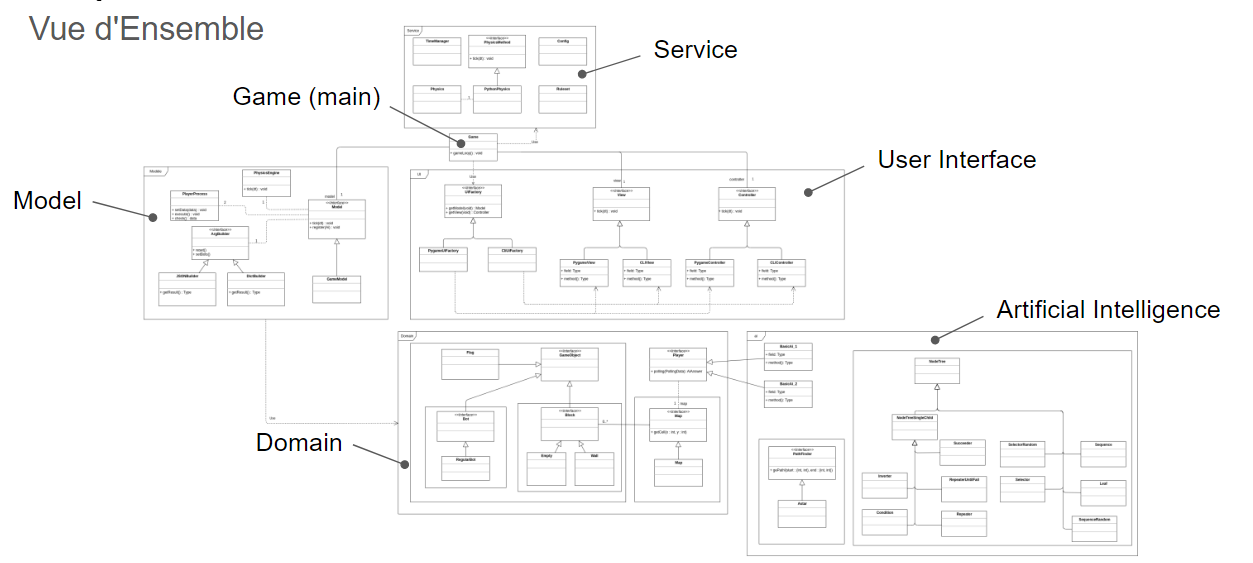
\includegraphics[scale=0.52,angle=90]{data/archi/vue_ensemble.png}{}
    \caption{Vue d'ensemble de l'architecture, chaque élément est précisé dans les points suivants}
\end{figure}

\clearpage
\subsection{Service}

\begin{figure}[H]
    \centering
    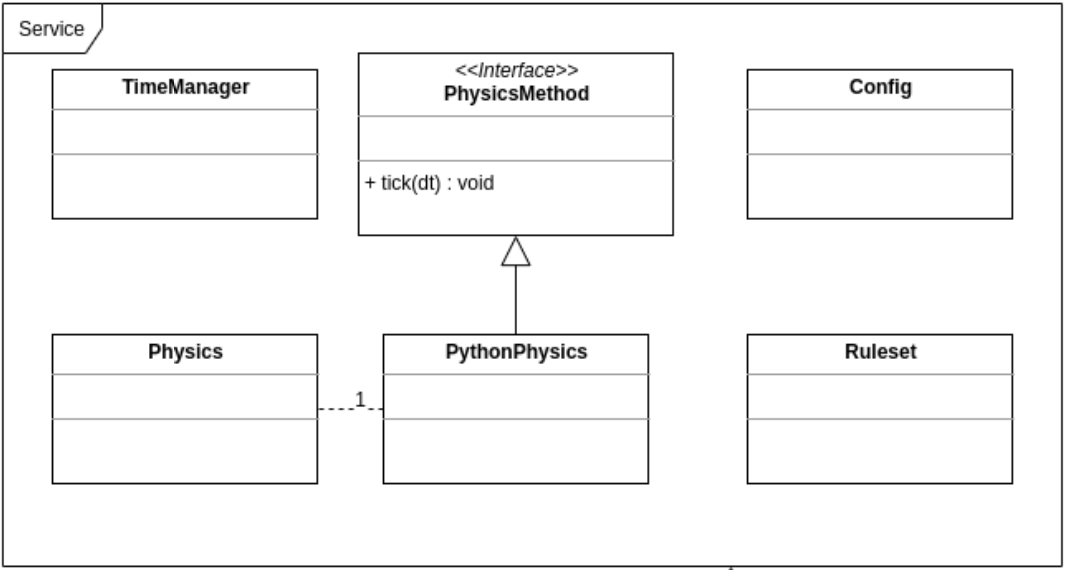
\includegraphics[scale=0.55]{data/archi/service.png}
    \caption{Package Service}
\end{figure}

Service est un package indépendant dans lequel nous avons créé des utilitaires plus ou moins centrés sur le cas particulier du jeu. Ils sont accessible partout dans le code.

\subsubsection{Config, Ruleset}

Ces deux classes, très similaires, sont un exemple de classe centrée sur le jeu. Elles permettent respectivement de gérer un fichier de configuration pour des paramètres ou des règles de jeu. Leur utilité est d'offrir un paramétrage par défaut, la création d'un fichier de configuration automatique avec les valeurs par défaut si il n'existe pas ou bien la complétion de paramètres manquants, puis un accès aux paramètres en lecture et en écriture.

\subsubsection{Physics, PhysicsMethod}

A l'opposé en terme de particularité, ces classes servent à implémenter des méthodes calculatoires génériques tout en gardant la main sur la technologie utilisée. Par défaut, nous utilisons l'implémentation PythonPhysics.

\subsubsection{TimeManager}

Cette classe sert à mesurer ou manipuler des données de temps comme par exemple chronométrer ou passer le temps jusqu'à un prochain tour.

\subsection{Partie Moteur de jeu}

\subsubsection{Domain}

\begin{figure}[H]
    \centering
    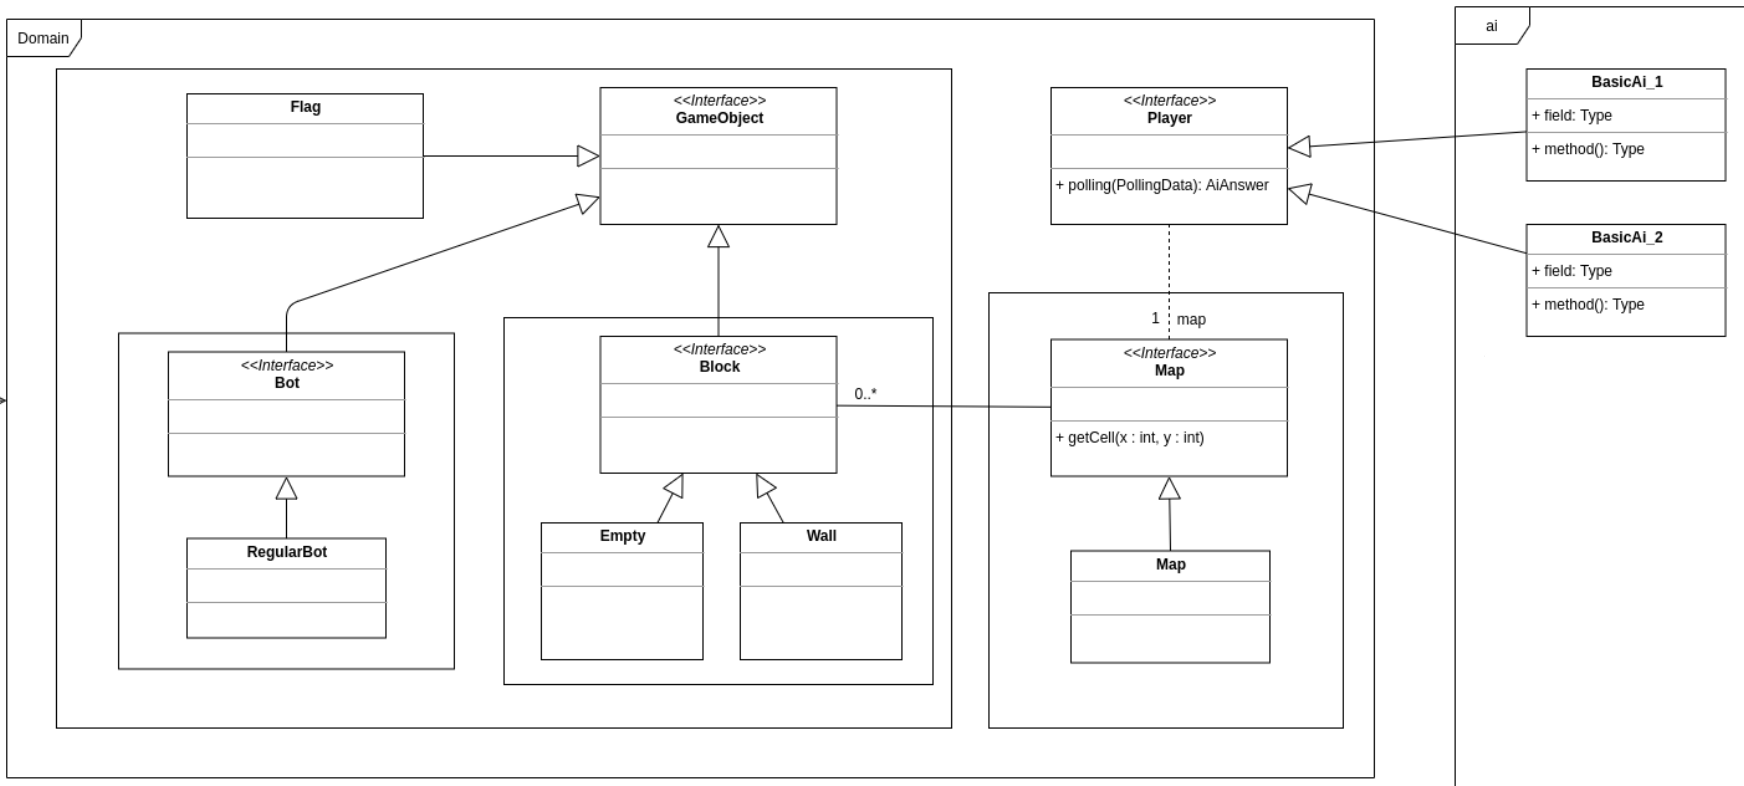
\includegraphics[scale=0.35]{data/archi/domain.png}
    \caption{Package Domain}
\end{figure}

Ce package contient des classes de description des données tel que la carte, ses blocks et ses objects, les différents Bots à contrôler ainsi que le joueur les contrôlant.\\

Elle est très utilisée par le modèle du moteur de jeu et sa définition est connue par les joueurs qui peuvent s'en servir pour former leur propre représentation s'ils le souhaitent, grâce aux données qui leur sont communiquées à chaque tour.

\subsubsection{Model}

\begin{figure}[H]
    \centering
    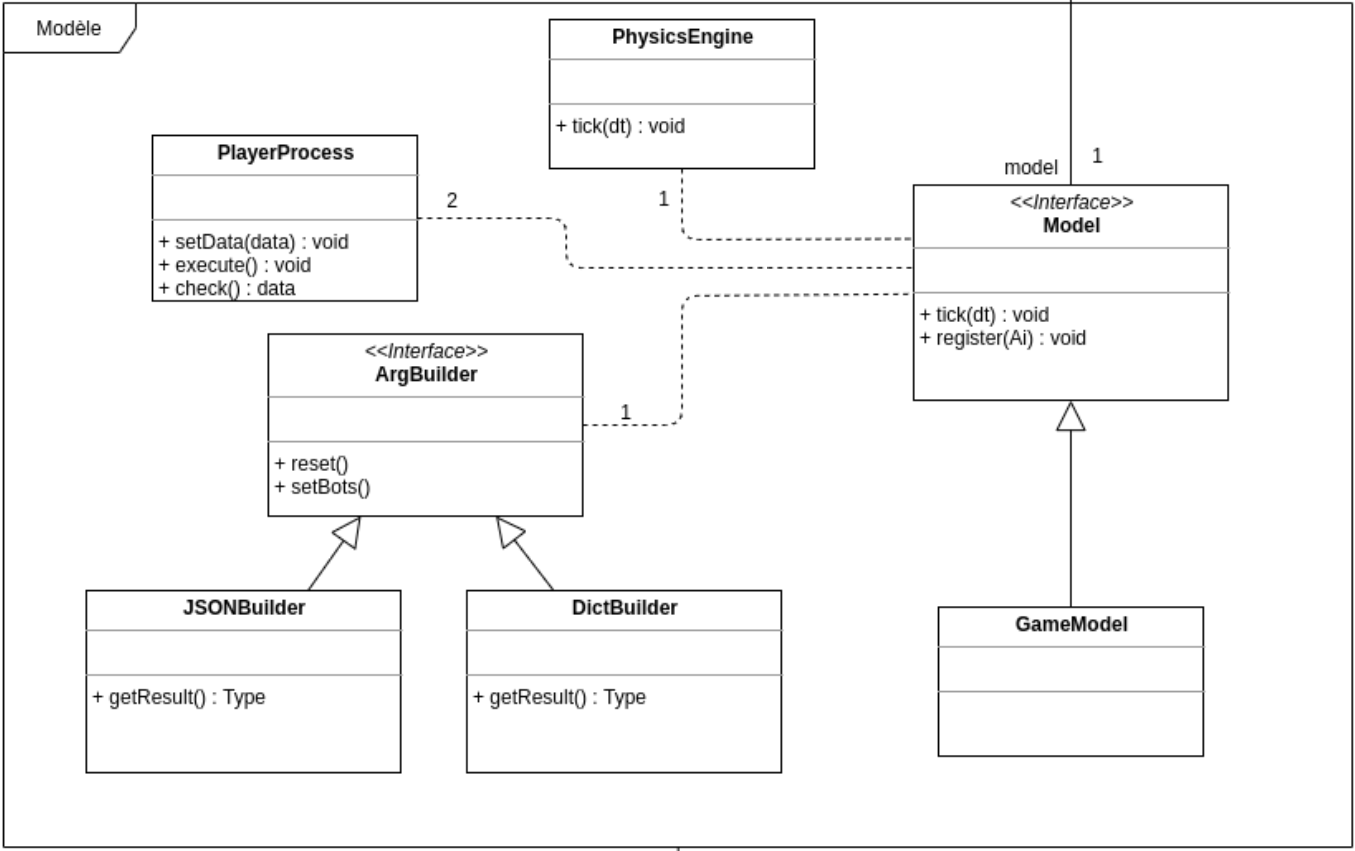
\includegraphics[scale=0.35]{data/archi/model.png}
    \caption{Package Model}
\end{figure}

C'est le package sur laquelle le jeu se base pour gérer les tours. Il contient le modèle à qui on demande d'initialiser et d'entretenir tous les éléments présents sur la carte, y compris les joueurs.\\

Le modèle interagit avec le moteur physique qui l'aide à prendre les bonnes décisions en terme de déplacements, interactions physiques et autres calculs. Il contient et gère deux PlayerProcess qui seront l'environnement dans lequel évolueront les IA. Enfin, il utiliser un ArgBuilder afin de correctement formaliser les données qui seront envoyées aux PlayerProcess.\\

Pour entrer dans plus de détails concernant PlayerProcess, c'est une simple implémentation de Process qui lance la fonction de polling d'un Player lorsque le modèle lui envoie les données d'un nouveau tour dans une queue. Le modèle récupère le retour à la fin du temps imparti pour ce tour. De cette manière, les IA ne peuvent pas directement impacter la performance du moteur de jeu en utilisant tout le temps processeur : ce serait son propre temps processeur.

\subsubsection{User Interface}

\begin{figure}[H]
    \centering
    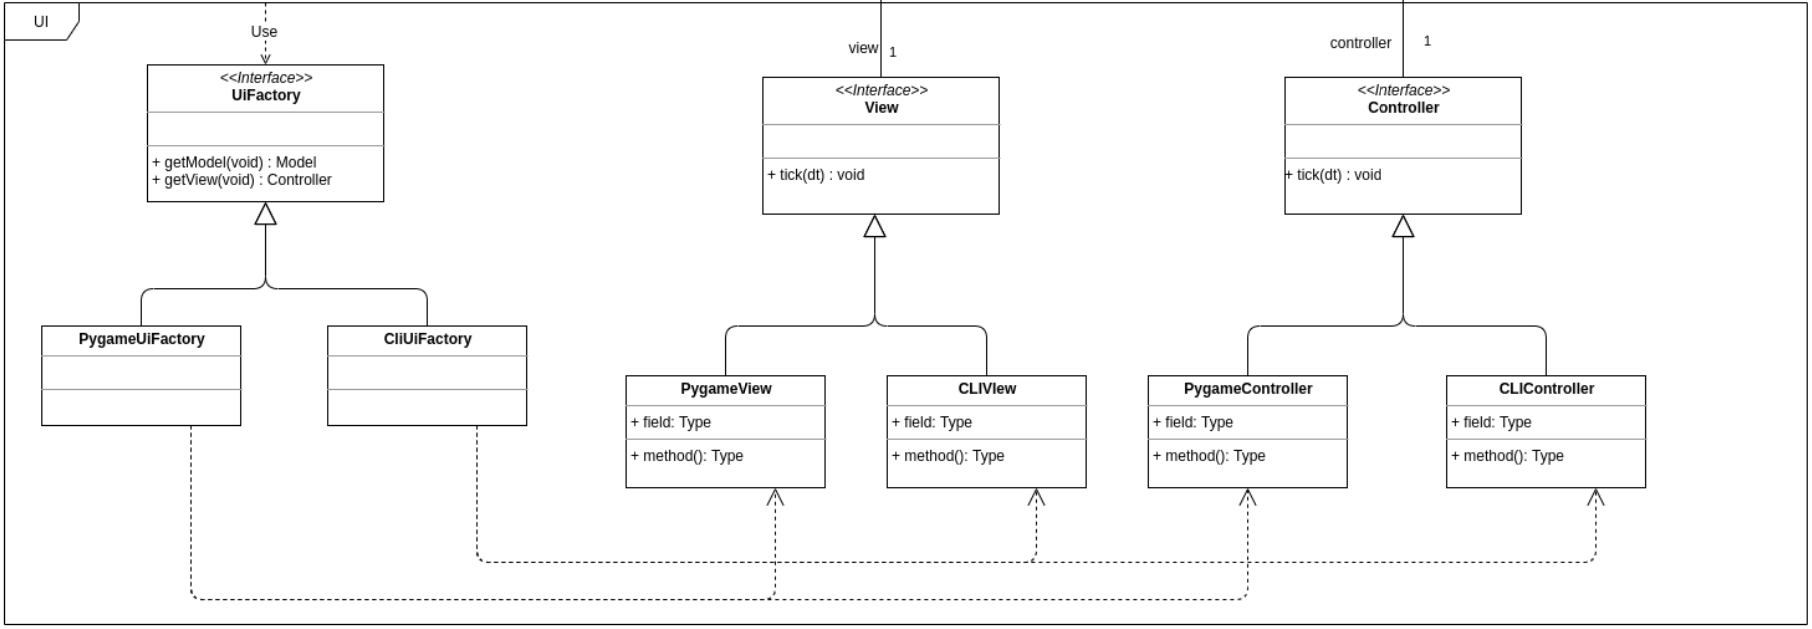
\includegraphics[scale=0.35]{data/archi/ui.png}
    \caption{Package User Interface}
\end{figure}

Ce package est une factory d'interface view/controller utilisée par le jeu. Ceux-ci sont simplement appelés à chaque tour de jeu et ont la possibilité d'intéragir avec le modèle.\\

Dans notre implémentation, on dispose de la vue Pygame (graphique avec des contrôles de debug) et de la vue en CLI (minimaliste mais permet de ne pas "gaspiller" de temps pour une interface).

\newpage
\subsection{Partie IA}
Tout d'abord, l'architecture pour les codes relatifs à l'IA est décomposée en trois sous-parties étant:
\begin{itemize}
    \item Un package PlayerTest où différentes IA sont implémentés.
    \item Un package BehaviorTree relatif aux arbres de comportements.
    \item Un package Pathfinding pour la recherche de chemin utilisées pour les déplacements.
    \\
\end{itemize}{}

\subsection{Behavior Tree}

\begin{figure}[H]
    \centering
    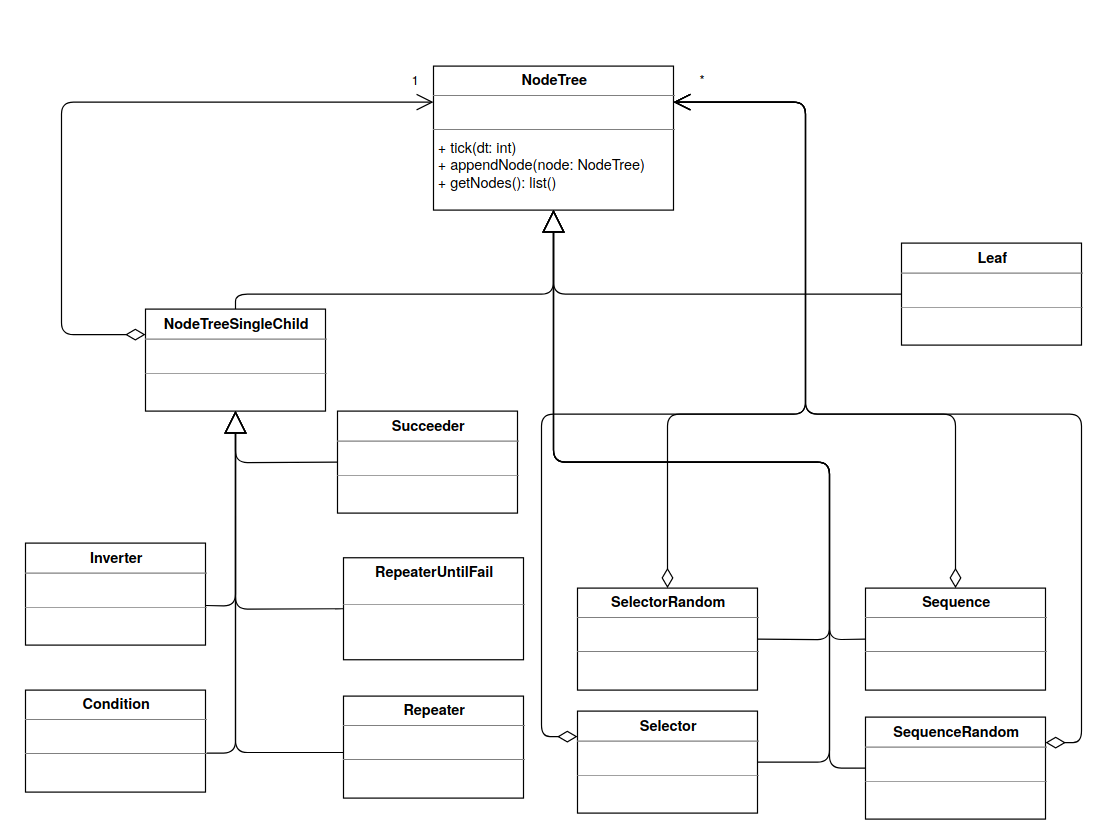
\includegraphics[scale=0.3]{data/archi/archi_nodetree.png}
    \caption{Architecture Behavior Tree}
    \label{}
\end{figure}

L'ia va reposer sur un arbre de comportement, qui est un automate, mais avec une hiérarchisation des noeuds. Chaque noeud peut posséder ou non des enfants. Chaque type de noeud redéfini la méthode \textit{tick()}, qui permet d'avancer dans l'arbre.\\
Chaque noeud doit renvoyer une valeur parmi ces trois : \textit{SUCCESS}, \textit{FAILURE} ou \textit{RUNNING}.\\
Les noeuds possède une mémoire pour se souvenir du noeud en cours d'exécution, pour pouvoir reprendre son exécution lors du prochain tick.

Nous utilisons donc le pattern composite pour cette partie de l'architecture. \textit{NodeTree} est donc l'interface qui permet la gestion des noeurs enfants. Trois types de noeuds implémente cette interface. \textit{NodeTreeSingleChild} et ses dérivés sont des noeuds ne pouvant posséder qu'un seul enfant. En cas de tentative d'ajout, une exception est levée.\\
Il y a ensuite \textit{Leaf}, qui est la feuille de l'arbre. Cette feuille prend dans son constructeur un pointeur vers la fonction qui sera appelée lors du \textit{tick()}. Comme pour \textit{NodeTreeSingleChild}, une tentative d'ajout d'un noeud lève un exception, une feuille ne pouvant avoir de fils.\\
Il y a ensuite tous les autre noeuds, qui n'ont rien de particulier dans la gestion des enfants, seul la fonction \textit{tick()} est redéfinie.

\subsubsection{Pathfinding}

\begin{figure}[H]
    \centering
    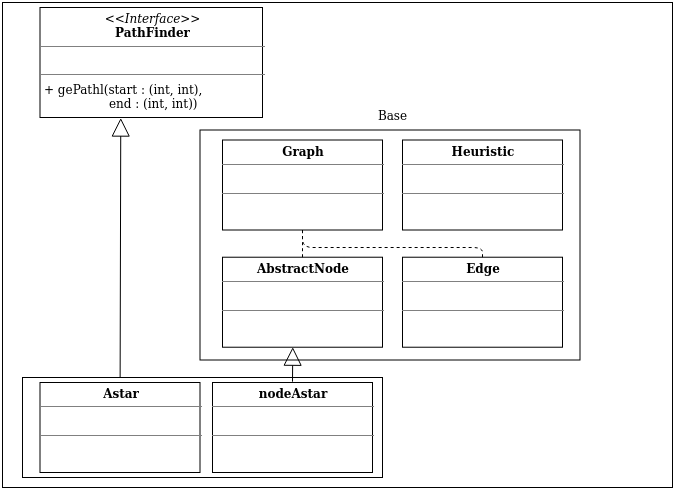
\includegraphics[scale=0.7]{data/pathfindingArchi.png}
    \caption{Architecture Pathinding}
    \label{}
\end{figure}
Pour la package Pathfinding, nous avons organisé de manière à ce que n'importe quel algorithme de recherche de chemin puisse être implémenté et utilisé sans avoir à modifier le code des joueurs mise à part la sélection de l'algorithme.

Nous avons d'une part le package Base où tout outil nécessaire à la création de chemin a été généralisé, c'est à dire une classe pour les noeuds abstraite que chaque algorithme pourra hériter selon ses besoins, une classe pour arête et graphe ainsi qu'une interface pathfinder avec une seule méthode getPath pour récupérer le chemin calculé.

Chaque algorithme de pathfinding doit hérité et utilisé cette base, par exemple pour l'algorithme A*, nous avons la classe Astar qui implémente pathFinder ainsi que NodeAstar qui implémente la classe pour les noeuds (Abstract Node).
\\
Tout ajout d'algorithme de pathfinding se fera par la création d'un package relatif à ce pathfinding, avec deux classes minimum, une implémentant la représentation abstraite des noeuds, et une implémentant l'interface pathfinder, c'est à dire une classe avec une fonction getPath permettant de renvoyer le chemin calculé (une liste de points).

Cette représentation permet d'ajouter facilement n'importe quel algorithme de recherche de chemin sans avoir à perturber le fonctionnement des autres instances tout en permettant de mettre tout le monde d'accord sur quelle est la représentation d'un noeud, graphe, arête...
\\

Pour le package PlayerTest, toute nouvelle IA ou nouveau joueur devant être implémenté doit hériter de la classe Player du domaine, étant le contrat à respecter pour pouvoir communiquer avec le moteur de jeu, c'est à dire pouvoir recevoir des informations sur l'évolution de la partie et en retour pouvoir envoyer nos prochaines actions que le moteur de jeu doit effectuer.
La classe MyLittlePlayer représente une IA avec arbre de comportement et se déplaçant à l'aide de l'algorithme A*.\\
La classe MyPlayerAstar représente une IA sans arbre de comportement se déplaçant avec A*.